%% Supplementary material for the TimeTrack FGCS manuscript
\documentclass[a4paper,11pt]{article}
\usepackage[margin=1in]{geometry}
\usepackage{booktabs,graphicx,hyperref,amsmath}

\title{Supplementary Material:\\
Hierarchy-Aware Forecast Reconciliation for Multi-Level Cloud Telemetry}
\author{Abdelhak Kadouma \and Amit Shukla \and Mohammed Elmusrati}
\date{}

\begin{document}
\maketitle

\section{Purpose}
This supplement collects the full claim matrix, extended bootstrap forest,
memory accuracy-versus-horizon plot, and pointers to seed/peak CSV grids.
All numbers derive from \texttt{final-reporting-freeze-v2} aggregate artifacts.

\section{Full claim-support matrix}
\input{claim_support_full}

\section{Extended bootstrap comparisons}
\begin{figure}[h]
\centering
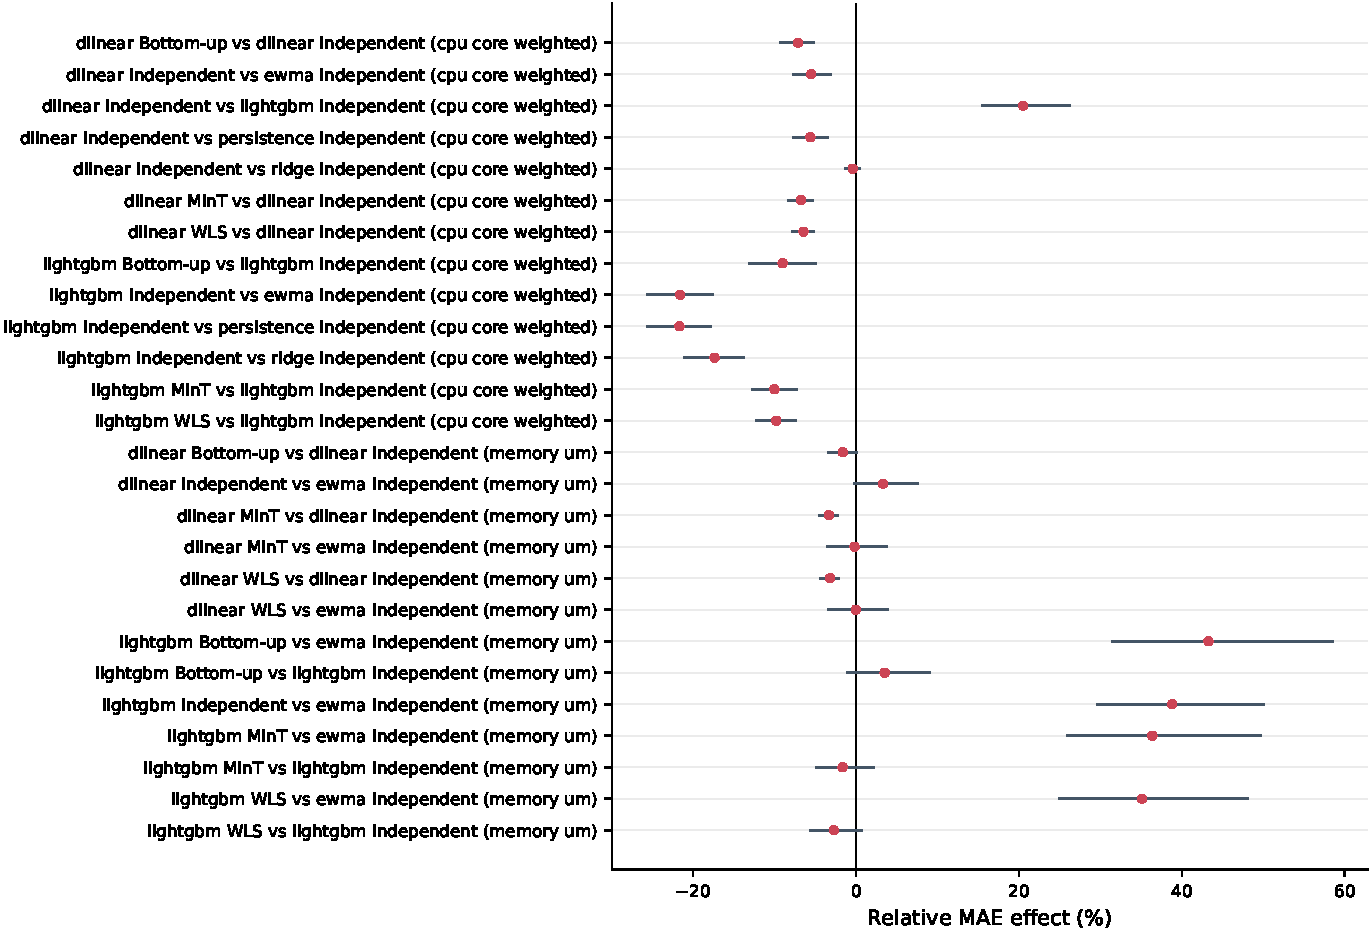
\includegraphics[width=0.98\textwidth]{../figs/supplementary/bootstrap_relative_effects_full.pdf}
\caption{Extended robustness relative-effect forest plot.}
\end{figure}

\section{Memory accuracy versus horizon}
\begin{figure}[h]
\centering

\includegraphics[width=0.7\textwidth]{../figs/supplementary/memory_accuracy_vs_horizon.pdf}
\caption{Memory MAE versus horizon for selected model--method pairs.}
\end{figure}

\section{CSV grids}
Full seed-by-fold-by-horizon tables:
\texttt{results/main/table05\_seed\_robustness.csv}.\\
Peak matrices:
\texttt{results/main/table08\_peak\_operational\_evidence.csv}.\\
Statistical families:
\texttt{results/main/table06\_final\_statistical\_evidence.csv}.

\end{document}
